% Created by tikzDevice version 0.12.6 on 2024-10-23 19:34:51
% !TEX encoding = UTF-8 Unicode
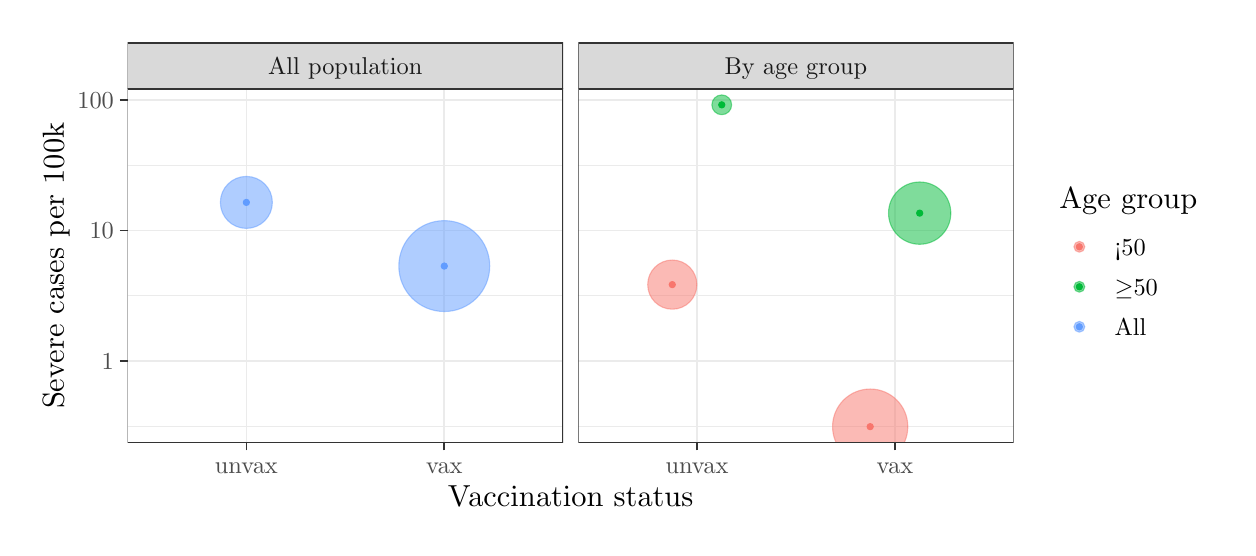
\begin{tikzpicture}[x=1pt,y=1pt]
\definecolor{fillColor}{RGB}{255,255,255}
\path[use as bounding box,fill=fillColor,fill opacity=0.00] (0,0) rectangle (433.62,180.67);
\begin{scope}
\path[clip] (  0.00,  0.00) rectangle (433.62,180.67);
\definecolor{drawColor}{RGB}{255,255,255}
\definecolor{fillColor}{RGB}{255,255,255}

\path[draw=drawColor,line width= 0.6pt,line join=round,line cap=round,fill=fillColor] (  0.00,  0.00) rectangle (433.62,180.68);
\end{scope}
\begin{scope}
\path[clip] ( 36.11, 30.69) rectangle (193.45,158.60);
\definecolor{fillColor}{RGB}{255,255,255}

\path[fill=fillColor] ( 36.11, 30.69) rectangle (193.45,158.60);
\definecolor{drawColor}{gray}{0.92}

\path[draw=drawColor,line width= 0.3pt,line join=round] ( 36.11, 36.63) --
	(193.45, 36.63);

\path[draw=drawColor,line width= 0.3pt,line join=round] ( 36.11, 83.79) --
	(193.45, 83.79);

\path[draw=drawColor,line width= 0.3pt,line join=round] ( 36.11,130.94) --
	(193.45,130.94);

\path[draw=drawColor,line width= 0.6pt,line join=round] ( 36.11, 60.21) --
	(193.45, 60.21);

\path[draw=drawColor,line width= 0.6pt,line join=round] ( 36.11,107.36) --
	(193.45,107.36);

\path[draw=drawColor,line width= 0.6pt,line join=round] ( 36.11,154.52) --
	(193.45,154.52);

\path[draw=drawColor,line width= 0.6pt,line join=round] ( 79.02, 30.69) --
	( 79.02,158.60);

\path[draw=drawColor,line width= 0.6pt,line join=round] (150.54, 30.69) --
	(150.54,158.60);
\definecolor{drawColor}{RGB}{97,156,255}
\definecolor{fillColor}{RGB}{97,156,255}

\path[draw=drawColor,draw opacity=0.50,line width= 0.4pt,line join=round,line cap=round,fill=fillColor,fill opacity=0.50] ( 79.02,117.53) circle (  9.39);

\path[draw=drawColor,draw opacity=0.50,line width= 0.4pt,line join=round,line cap=round,fill=fillColor,fill opacity=0.50] (150.54, 94.52) circle ( 16.42);
\definecolor{drawColor}{RGB}{97,156,255}
\definecolor{fillColor}{RGB}{97,156,255}

\path[draw=drawColor,line width= 0.4pt,line join=round,line cap=round,fill=fillColor] ( 79.02,117.53) circle (  1.11);

\path[draw=drawColor,line width= 0.4pt,line join=round,line cap=round,fill=fillColor] (150.54, 94.52) circle (  1.11);
\definecolor{drawColor}{gray}{0.20}

\path[draw=drawColor,line width= 0.6pt,line join=round,line cap=round] ( 36.11, 30.69) rectangle (193.45,158.60);
\end{scope}
\begin{scope}
\path[clip] (198.95, 30.69) rectangle (356.30,158.60);
\definecolor{fillColor}{RGB}{255,255,255}

\path[fill=fillColor] (198.95, 30.69) rectangle (356.30,158.60);
\definecolor{drawColor}{gray}{0.92}

\path[draw=drawColor,line width= 0.3pt,line join=round] (198.95, 36.63) --
	(356.30, 36.63);

\path[draw=drawColor,line width= 0.3pt,line join=round] (198.95, 83.79) --
	(356.30, 83.79);

\path[draw=drawColor,line width= 0.3pt,line join=round] (198.95,130.94) --
	(356.30,130.94);

\path[draw=drawColor,line width= 0.6pt,line join=round] (198.95, 60.21) --
	(356.30, 60.21);

\path[draw=drawColor,line width= 0.6pt,line join=round] (198.95,107.36) --
	(356.30,107.36);

\path[draw=drawColor,line width= 0.6pt,line join=round] (198.95,154.52) --
	(356.30,154.52);

\path[draw=drawColor,line width= 0.6pt,line join=round] (241.87, 30.69) --
	(241.87,158.60);

\path[draw=drawColor,line width= 0.6pt,line join=round] (313.38, 30.69) --
	(313.38,158.60);
\definecolor{drawColor}{RGB}{248,118,109}
\definecolor{fillColor}{RGB}{248,118,109}

\path[draw=drawColor,draw opacity=0.50,line width= 0.4pt,line join=round,line cap=round,fill=fillColor,fill opacity=0.50] (232.93, 87.82) circle (  8.88);

\path[draw=drawColor,draw opacity=0.50,line width= 0.4pt,line join=round,line cap=round,fill=fillColor,fill opacity=0.50] (304.44, 36.50) circle ( 13.59);
\definecolor{drawColor}{RGB}{0,186,56}
\definecolor{fillColor}{RGB}{0,186,56}

\path[draw=drawColor,draw opacity=0.50,line width= 0.4pt,line join=round,line cap=round,fill=fillColor,fill opacity=0.50] (250.80,152.79) circle (  3.57);

\path[draw=drawColor,draw opacity=0.50,line width= 0.4pt,line join=round,line cap=round,fill=fillColor,fill opacity=0.50] (322.32,113.65) circle ( 11.25);
\definecolor{drawColor}{RGB}{248,118,109}
\definecolor{fillColor}{RGB}{248,118,109}

\path[draw=drawColor,line width= 0.4pt,line join=round,line cap=round,fill=fillColor] (232.93, 87.82) circle (  1.11);

\path[draw=drawColor,line width= 0.4pt,line join=round,line cap=round,fill=fillColor] (304.44, 36.50) circle (  1.11);
\definecolor{drawColor}{RGB}{0,186,56}
\definecolor{fillColor}{RGB}{0,186,56}

\path[draw=drawColor,line width= 0.4pt,line join=round,line cap=round,fill=fillColor] (250.80,152.79) circle (  1.11);

\path[draw=drawColor,line width= 0.4pt,line join=round,line cap=round,fill=fillColor] (322.32,113.65) circle (  1.11);
\definecolor{drawColor}{gray}{0.20}

\path[draw=drawColor,line width= 0.6pt,line join=round,line cap=round] (198.95, 30.69) rectangle (356.30,158.60);
\end{scope}
\begin{scope}
\path[clip] ( 36.11,158.60) rectangle (193.45,175.17);
\definecolor{drawColor}{gray}{0.20}
\definecolor{fillColor}{gray}{0.85}

\path[draw=drawColor,line width= 0.6pt,line join=round,line cap=round,fill=fillColor] ( 36.11,158.60) rectangle (193.45,175.18);
\definecolor{drawColor}{gray}{0.10}

\node[text=drawColor,anchor=base,inner sep=0pt, outer sep=0pt, scale=  0.88] at (114.78,163.86) {All population};
\end{scope}
\begin{scope}
\path[clip] (198.95,158.60) rectangle (356.30,175.17);
\definecolor{drawColor}{gray}{0.20}
\definecolor{fillColor}{gray}{0.85}

\path[draw=drawColor,line width= 0.6pt,line join=round,line cap=round,fill=fillColor] (198.95,158.60) rectangle (356.30,175.18);
\definecolor{drawColor}{gray}{0.10}

\node[text=drawColor,anchor=base,inner sep=0pt, outer sep=0pt, scale=  0.88] at (277.62,163.86) {By age group};
\end{scope}
\begin{scope}
\path[clip] (  0.00,  0.00) rectangle (433.62,180.67);
\definecolor{drawColor}{gray}{0.20}

\path[draw=drawColor,line width= 0.6pt,line join=round] ( 79.02, 27.94) --
	( 79.02, 30.69);

\path[draw=drawColor,line width= 0.6pt,line join=round] (150.54, 27.94) --
	(150.54, 30.69);
\end{scope}
\begin{scope}
\path[clip] (  0.00,  0.00) rectangle (433.62,180.67);
\definecolor{drawColor}{gray}{0.30}

\node[text=drawColor,anchor=base,inner sep=0pt, outer sep=0pt, scale=  0.88] at ( 79.02, 19.68) {unvax};

\node[text=drawColor,anchor=base,inner sep=0pt, outer sep=0pt, scale=  0.88] at (150.54, 19.68) {vax};
\end{scope}
\begin{scope}
\path[clip] (  0.00,  0.00) rectangle (433.62,180.67);
\definecolor{drawColor}{gray}{0.20}

\path[draw=drawColor,line width= 0.6pt,line join=round] (241.87, 27.94) --
	(241.87, 30.69);

\path[draw=drawColor,line width= 0.6pt,line join=round] (313.38, 27.94) --
	(313.38, 30.69);
\end{scope}
\begin{scope}
\path[clip] (  0.00,  0.00) rectangle (433.62,180.67);
\definecolor{drawColor}{gray}{0.30}

\node[text=drawColor,anchor=base,inner sep=0pt, outer sep=0pt, scale=  0.88] at (241.87, 19.68) {unvax};

\node[text=drawColor,anchor=base,inner sep=0pt, outer sep=0pt, scale=  0.88] at (313.38, 19.68) {vax};
\end{scope}
\begin{scope}
\path[clip] (  0.00,  0.00) rectangle (433.62,180.67);
\definecolor{drawColor}{gray}{0.30}

\node[text=drawColor,anchor=base east,inner sep=0pt, outer sep=0pt, scale=  0.88] at ( 31.16, 57.18) {1};

\node[text=drawColor,anchor=base east,inner sep=0pt, outer sep=0pt, scale=  0.88] at ( 31.16,104.33) {10};

\node[text=drawColor,anchor=base east,inner sep=0pt, outer sep=0pt, scale=  0.88] at ( 31.16,151.49) {100};
\end{scope}
\begin{scope}
\path[clip] (  0.00,  0.00) rectangle (433.62,180.67);
\definecolor{drawColor}{gray}{0.20}

\path[draw=drawColor,line width= 0.6pt,line join=round] ( 33.36, 60.21) --
	( 36.11, 60.21);

\path[draw=drawColor,line width= 0.6pt,line join=round] ( 33.36,107.36) --
	( 36.11,107.36);

\path[draw=drawColor,line width= 0.6pt,line join=round] ( 33.36,154.52) --
	( 36.11,154.52);
\end{scope}
\begin{scope}
\path[clip] (  0.00,  0.00) rectangle (433.62,180.67);
\definecolor{drawColor}{RGB}{0,0,0}

\node[text=drawColor,anchor=base,inner sep=0pt, outer sep=0pt, scale=  1.10] at (196.20,  7.64) {Vaccination status};
\end{scope}
\begin{scope}
\path[clip] (  0.00,  0.00) rectangle (433.62,180.67);
\definecolor{drawColor}{RGB}{0,0,0}

\node[text=drawColor,rotate= 90.00,anchor=base,inner sep=0pt, outer sep=0pt, scale=  1.10] at ( 13.08, 94.64) {Severe cases per 100k};
\end{scope}
\begin{scope}
\path[clip] (  0.00,  0.00) rectangle (433.62,180.67);
\definecolor{fillColor}{RGB}{255,255,255}

\path[fill=fillColor] (367.30, 59.86) rectangle (428.12,129.43);
\end{scope}
\begin{scope}
\path[clip] (  0.00,  0.00) rectangle (433.62,180.67);
\definecolor{drawColor}{RGB}{0,0,0}

\node[text=drawColor,anchor=base west,inner sep=0pt, outer sep=0pt, scale=  1.10] at (372.80,115.29) {Age group};
\end{scope}
\begin{scope}
\path[clip] (  0.00,  0.00) rectangle (433.62,180.67);
\definecolor{fillColor}{RGB}{255,255,255}

\path[fill=fillColor] (372.80, 94.26) rectangle (387.25,108.72);
\end{scope}
\begin{scope}
\path[clip] (  0.00,  0.00) rectangle (433.62,180.67);
\definecolor{drawColor}{RGB}{248,118,109}
\definecolor{fillColor}{RGB}{248,118,109}

\path[draw=drawColor,draw opacity=0.50,line width= 0.4pt,line join=round,line cap=round,fill=fillColor,fill opacity=0.50] (380.02,101.49) circle (  1.96);
\end{scope}
\begin{scope}
\path[clip] (  0.00,  0.00) rectangle (433.62,180.67);
\definecolor{drawColor}{RGB}{248,118,109}
\definecolor{fillColor}{RGB}{248,118,109}

\path[draw=drawColor,line width= 0.4pt,line join=round,line cap=round,fill=fillColor] (380.02,101.49) circle (  1.11);
\end{scope}
\begin{scope}
\path[clip] (  0.00,  0.00) rectangle (433.62,180.67);
\definecolor{fillColor}{RGB}{255,255,255}

\path[fill=fillColor] (372.80, 79.81) rectangle (387.25, 94.26);
\end{scope}
\begin{scope}
\path[clip] (  0.00,  0.00) rectangle (433.62,180.67);
\definecolor{drawColor}{RGB}{0,186,56}
\definecolor{fillColor}{RGB}{0,186,56}

\path[draw=drawColor,draw opacity=0.50,line width= 0.4pt,line join=round,line cap=round,fill=fillColor,fill opacity=0.50] (380.02, 87.04) circle (  1.96);
\end{scope}
\begin{scope}
\path[clip] (  0.00,  0.00) rectangle (433.62,180.67);
\definecolor{drawColor}{RGB}{0,186,56}
\definecolor{fillColor}{RGB}{0,186,56}

\path[draw=drawColor,line width= 0.4pt,line join=round,line cap=round,fill=fillColor] (380.02, 87.04) circle (  1.11);
\end{scope}
\begin{scope}
\path[clip] (  0.00,  0.00) rectangle (433.62,180.67);
\definecolor{fillColor}{RGB}{255,255,255}

\path[fill=fillColor] (372.80, 65.36) rectangle (387.25, 79.81);
\end{scope}
\begin{scope}
\path[clip] (  0.00,  0.00) rectangle (433.62,180.67);
\definecolor{drawColor}{RGB}{97,156,255}
\definecolor{fillColor}{RGB}{97,156,255}

\path[draw=drawColor,draw opacity=0.50,line width= 0.4pt,line join=round,line cap=round,fill=fillColor,fill opacity=0.50] (380.02, 72.58) circle (  1.96);
\end{scope}
\begin{scope}
\path[clip] (  0.00,  0.00) rectangle (433.62,180.67);
\definecolor{drawColor}{RGB}{97,156,255}
\definecolor{fillColor}{RGB}{97,156,255}

\path[draw=drawColor,line width= 0.4pt,line join=round,line cap=round,fill=fillColor] (380.02, 72.58) circle (  1.11);
\end{scope}
\begin{scope}
\path[clip] (  0.00,  0.00) rectangle (433.62,180.67);
\definecolor{drawColor}{RGB}{0,0,0}

\node[text=drawColor,anchor=base west,inner sep=0pt, outer sep=0pt, scale=  0.88] at (392.75, 98.46) {<50};
\end{scope}
\begin{scope}
\path[clip] (  0.00,  0.00) rectangle (433.62,180.67);
\definecolor{drawColor}{RGB}{0,0,0}

\node[text=drawColor,anchor=base west,inner sep=0pt, outer sep=0pt, scale=  0.88] at (392.75, 84.01) {$\geq$50};
\end{scope}
\begin{scope}
\path[clip] (  0.00,  0.00) rectangle (433.62,180.67);
\definecolor{drawColor}{RGB}{0,0,0}

\node[text=drawColor,anchor=base west,inner sep=0pt, outer sep=0pt, scale=  0.88] at (392.75, 69.55) {All};
\end{scope}
\end{tikzpicture}
